\documentclass[11pt]{article}
\usepackage[margin=1in]{geometry}
\usepackage{amsmath,amssymb,amsthm}
\usepackage{graphicx}
\usepackage[hidelinks]{hyperref}

\newtheorem*{theorem}{Theorem}

\newcommand{\F}{\mathcal{F}}
\newcommand{\Hh}{\mathbb{H}}
\newcommand{\R}{\mathbb{R}}
\newcommand{\LF}{\operatorname{LF}}

\title{Literature Answer: The Hyperbolic-Space Free Space Question of Doucha--Kaufmann}
\author{Run \texttt{fa\_banach\_001}, agent \texttt{agent\_lane\_00}}
\date{June 18, 2026}

\begin{document}
\maketitle

\section*{Status}

\textbf{Packet type:} literature answer already present in later literature.

\textbf{Verdict:} Gartland's arXiv:2406.10986 proves
\[
  \LF(\Hh^n)\simeq \LF(\R^n)
\]
for hyperbolic \(n\)-space. This gives a positive answer to the isomorphism
clause of Doucha--Kaufmann's Question 6. Since \(\F(\R^n)\) has a Schauder
basis by H\'ajek--Perneck\'a, it also gives a positive answer to the
Schauder-basis clause.

\section*{Source Metadata}

\textbf{Original source.}
Michal Doucha and Pedro L. Kaufmann, \emph{Approximation properties in
Lipschitz-free spaces over groups}, arXiv:2005.09785v2.

\textbf{Supporting answer source.}
Chris Gartland, \emph{Hyperbolic Metric Spaces and Stochastic Embeddings},
arXiv:2406.10986v2.

\textbf{Basis input.}
Petr H\'ajek and Eva Perneck\'a, \emph{On Schauder bases in Lipschitz-free
spaces}, J. Math. Anal. Appl. 416 (2014), 629--646.

\section*{Open Question}

After proving that every net \(N\subseteq\Hh^n\) has \(\F(N)\) with a
Schauder basis, Doucha--Kaufmann ask:

\begin{quote}
Does \(\F(\Hh^n)\) have the Schauder basis? Do we have
\(\F(\Hh^n)\simeq\F(\R^n)\)?
\end{quote}

\begin{center}

\includegraphics[width=0.95\linewidth]{figures/open_question_crop.png}
\end{center}

\section*{Supporting Answer}

Gartland's introduction states the answer as Theorem D, citing Corollary 6.4:

\begin{center}
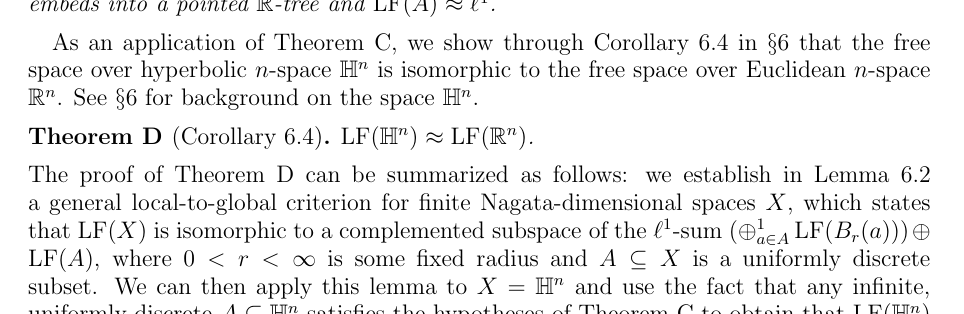
\includegraphics[width=0.95\linewidth]{figures/supporting_intro_crop.png}
\end{center}

The formal statement and proof appear as Corollary 6.4.

\begin{center}
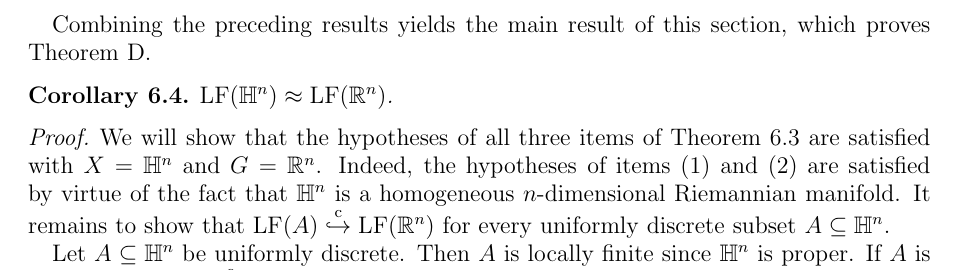
\includegraphics[width=0.95\linewidth]{figures/supporting_corollary_crop.png}
\end{center}

\section*{Formal Statement}

\begin{theorem}
For every integer \(n\ge 2\),
\[
  \F(\Hh^n)\simeq \F(\R^n).
\]
Consequently, \(\F(\Hh^n)\) has a Schauder basis.
\end{theorem}

\begin{proof}
Gartland proves in \cite[Corollary 6.4]{Gartland} that
\(\LF(\Hh^n)\simeq\LF(\R^n)\). Gartland's notation \(\LF(M)\) denotes the
Lipschitz-free space over \(M\), the same object denoted \(\F(M)\) by
Doucha--Kaufmann. Thus \(\F(\Hh^n)\simeq\F(\R^n)\).

By H\'ajek--Perneck\'a \cite{HP}, \(\F(\R^n)\) has a Schauder basis. Since
the existence of a Schauder basis is preserved under Banach-space isomorphism,
\(\F(\Hh^n)\) has a Schauder basis as well.
\end{proof}

\section*{Scope And Limitations}

Gartland states the result for \(2\le n\in\mathbb{N}\), the standard range for
real hyperbolic \(n\)-space in the cited proof. The \(n=1\) edge case is
trivial because the hyperbolic line is isometric to \(\R\).

The same source paper also reiterates the Candido--Cuth--Doucha question about
whether finitely generated hyperbolic groups have free space isomorphic to
\(\ell_1\). That adjacent question is already recorded in this run as
\path{solutions/literature_already_answered/1809.09957_hyperbolic_groups_free_space_l1/}
and is not duplicated here.

\section*{Search And Verification Notes}

The run indexes were searched for arXiv:2005.09785, arXiv:2406.10986,
hyperbolic-space phrases, and the core keywords ``Schauder basis'',
``Lipschitz-free'', and ``hyperbolic group''. No previous packet for the
\(\Hh^n\) clause was found. A separate existing packet already covers the
hyperbolic-group \(\ell_1\) clause.

\begin{thebibliography}{9}
\bibitem{DK}
M. Doucha and P. L. Kaufmann,
\emph{Approximation properties in Lipschitz-free spaces over groups},
arXiv:2005.09785.

\bibitem{Gartland}
C. Gartland,
\emph{Hyperbolic Metric Spaces and Stochastic Embeddings},
arXiv:2406.10986.

\bibitem{HP}
P. H\'ajek and E. Perneck\'a,
\emph{On Schauder bases in Lipschitz-free spaces},
J. Math. Anal. Appl. 416 (2014), 629--646.
\end{thebibliography}

\end{document}
